\chapter{Introduction}
\label{Introduction}

Phages are small viruses on the order of 27-190nm that infect and lyse (kill) specific bacteria, acting as nature's natural anti-microbial defense. 
Researchers are attempting to determine how phages can be used in various medical and industrial applications to control bacterial growth. 
However, researchers need to know how the interactions between phages and bacteria work in order to implement a robust method to control bacterial growth. \newline 

\section{Biological Background}
Phages are small viruses on the order of 27-190nm that infect and lyse (kill) specific bacteria.
The phage cycle process starts with a phage coming into contact with a bacterium.
Once it has identified an injection site, the phage can inject a strain of DNA into the bacteria.
The DNA strand has two options: it can either merge into the bacterial DNA, allowing the phage's DNA strand to replicate alongside the bacteria as they reproduce.
This process defines the Lysogenic cycle.
After a set amount of time, the DNA of the phage can unmerge and hijack the DNA replicating mechanism, creating multiple copies of itself, using the transcription, translation, and replication process to create multiple copies of itself.
The phages begin to self-assemble inside the bacteria until the bacteria is full of phages and explodes, the lysis stage, releasing the phages into the environment, ready to repeat the process again. 

This process can be visualized in \Cref{fig:phage_life_cycle} \cite{campbellFutureBacteriophageBiology2003}.
\begin{figure}
    \centering
    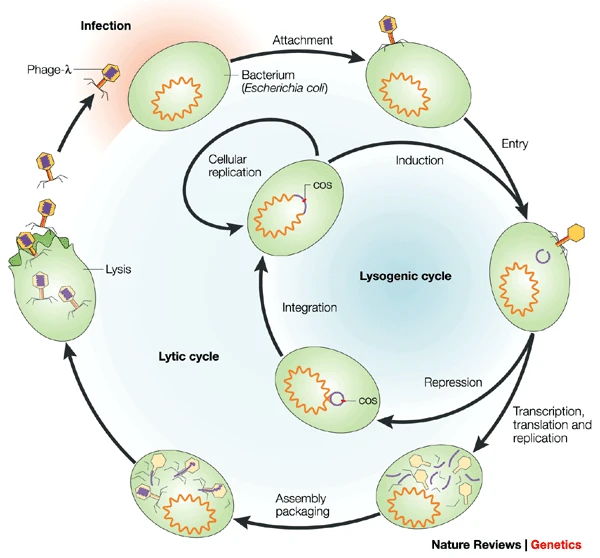
\includegraphics[width=0.5\linewidth]{Figures/phage_life_cycle.png}
    \caption{Life cycle of a phage, inside and outside a bacteria cell. Significant steps in the life cycle of a phage include the infection stage, integration, replication, and lysing process. Figure sourced from \citet{campbellFutureBacteriophageBiology2003}. }
    \label{fig:phage_life_cycle}
\end{figure}

\section{Phage Cocktail and Human Health}
There is particular interest in phage applications in human and animal health, called phage cocktail therapy, due to phages not exhibiting side effects.
Phage cocktails are a medicine that sick patients with bacterial diseases, such as \textit{Escherichia coli} can use. 
A patient can swallow a pill filled with a range of different phages that target \textit{E. coli}.
The phages will target the specific \textit{E. coli} bacteria, but it will not affect the other bacteria found in the gut of the human body and will not have any side effects on the body. 
There are 100 trillion microbes across 5,000 different types of bacteria strains in the human gut. 
Medicine such as antibiotics disrupt the intricate ecosystem of the gut microbiome, acting as a scorched-earth mechanism. 
Phages on the other hand specifically target a specific bacterial strain, acting as a sniper, with minimal to no effects to other bacteria, while penicillin acts as a bomb. 
A challenge that antibiotics face is that antibiotics create antibiotic resistant bacteria, meaning that the antibiotics is less effective in the future \cite{odonkorBacteriaResistanceAntibiotics2011, volkovaEffectsEarlylifePenicillin2021}. 
There is however hope that phage resistant bacteria become more susceptible to antibiotics due to changes in the cell structure \cite{laurePhageResistancemediatedTradeoffs2022, zhaoPhagedrivenCoevolutionReveals2024}. 

\section{Industrial Usage}
Phages have many uses in an industrial setting. 
Similarly, phage therapies can be used as a preventative method, by preventing the spread of common bacteria in livestock by dosing the animal feed with the phage pills. 
Farmers often raise livestock in tight spaces with a lack of sanitation facilities, increasing the risk of a disease spreading. \newline 
Phages can be used to control the growth of bacteria like \textit{Salmonella} while producing food in a factory \cite{sofferBacteriophagesSafelyReduce2016, kowalskaFreshVegetablesFruit2023}. 

\section{The Environment}
In an ecosystem like the ocean, the gut, or in soil, there are thousands of different microbes all interacting with one another or the surrounding environment.
The interactions are complex, with many factors affecting the growth of bacteria, fungi, phages, plants, animals, and more. 
Often, the interactions between agents in the environment are synergistic. 
When an animal dies, bacteria start to digest and decompose the animal into simpler chemicals like carbon and nitrogen that plants can use to grow, which is then eaten by other animals. \newline 

Not every interaction in the complex community can be identified, and if an interaction has been identified, the associated parameter values are unknown and need to be experimentally derived. 
External factors, such as flooding, droughts, chemical spills, or introduction of new agents have a massive impact on the ecosystem. 
These events can add or remove nutrients from the system, change environmental parameters such as the surrounding temperature, introduce competition, or create an imbalance in the population by killing agents. 
These effects can affect the larger ecosystem and food chain as a whole. 
Finally, phages can potentially be used to control cyanobacterial (blue-green algae) blooms in the environment and affect other agents such as plankton in the environment \cite{colomaFrequencyVirusresistantHosts2019}. 
With this, there is hope that water quality can be engineered without using harsh chemical processes what would otherwise pose environmental and health hazards \cite{tuckerIdentificationCyanophageMaLBP2005}. \newline
\newline

\section{Modelling Phages in a Complex Community}
Not much is known about phages in large and complex communities between other phages, bacteria, resources, and the environment. 
There have been previous attempts to model the complex dynamics of the populations between phages, bacteria, and resources, with the environment using Ordinary Differential Equations (ODE) and Delay Differential Equations (DDE).
however collecting the parameter values for the interactions is an expensive and laborious task, as the data has to experimentally collected in a lab. \newline 

A Resource-Phage-Bacteria system can be described as an $p\times b \times r$ system, meaning there are $p$ phages, $b$ bacteria, and $r$ resources arbitrarily interacting with one another. 
However, current modelling methods have mainly stayed with $1\times 1 \times 1$ models, meaning 1 phage, 1 bacteria, and 1 resource. \newline 

There are two main ways to model phage-bacteria dynamics: a spatial model and a non-spatial one.
A spatial model means that phages and bacteria can move through space and interact with their neighbors. 
Partial differential equations (PDE) and cellular agent based models have been created in an attempt to model spatial interactions.
Special considerations have to be accounted for with spatial models, such as bacteria and phages can only interact when they are in proximity to each other.
This creates areas of interaction and interest where agents are located, and areas of no interactions where there are no interactions.
Spatial models can potentially lead to more interesting and complex results but are limited to smaller populations and harder to develop. \newline 

Whereas in non-spatial models such as ODEs and DDEs, the bacteria and phages are assumed to be in a well-mixed solution and no distinction is made in regard to neighbors or distances to other agents. 
Interactions are simplified to a probabilistic approach, where only a percentage $p$ of bacteria and phages interact with one another at time step $t$.
Non non-spatial models are easier to develop and are more effective in modeling large populations, at the cost of losing spatial information. \newline
For this thesis, the focus will be modelling resource, phage, and bacteria interactions using an ODE model. 

\section{Thesis Project}
The project is divided into three logical parts, with an optional fourth part.
The first section is to create the network interaction. 
Here the user of the software can define the number of resources, phages, and bacteria, who interacts with who, and the strength and type of interactions. See \Cref{sec:part1} for further information. \newline
In part 2 (\Cref{sec:part2}), the user uploads the network model and parameters and as output receives the time data and population data as an array. \newline
Part 3 (\Cref{sec:part3}) allows the user to interact with part 1 and part 2 with a dashboard. 
The user can graphically edit the attribute values of the edges and nodes of the network, and the user can run more advanced visualizations, for example by changing a parameter value and seeing how that affects the population count. 
There are a few plots included out of the box that the user can test. 
The plots offered in part 3 offer interactivity like hiding and showing lines and dots, zooming in and out, and hovering over the lines and dots to show more details of the data. 
\newline
Finally, the user can optionally run multiple simulations and download the data to their disk to create their own custom visualizations using part 4 (\Cref{sec:part4}). 
The visualizations created in part 3 can theoretically be recreated in part 4. 
The user can choose the same parameter values used for a specific plot in part 3, run the simulation (under the "Ultimate Analysis" section (\Cref{sec:ultimate_analysis})), download the data, and reimplement the graphs. 